\chapter{System test}
This chapter presents the tests made through the project and optimization made to the product.

\section{Unit tests}
Each module was developed separately and then tested before adding more to the system. This made the process of combining all the blocks relatively smooth.\\
In this process we used uart a lot to debug. It is easy to use and provides a lot of insight when debugging. You can write specific messages on where in your code you are, or what values are in which registers etc.\\
When combining the blocks it is important to make sure everything is set up to use the same clock speeds and no pins overlap etc.

\section{Complete system test}
The Demoboard developed was a central part of the complete system test. The complete system test comprised of taking the demoboard outside, wait until it had good satellite connection and then note the GPS coordinates. We also compared the heading on the display compass with a compass on the mobile phone. Below is a picture of the test setup:
\begin{figure}[H]
\centering
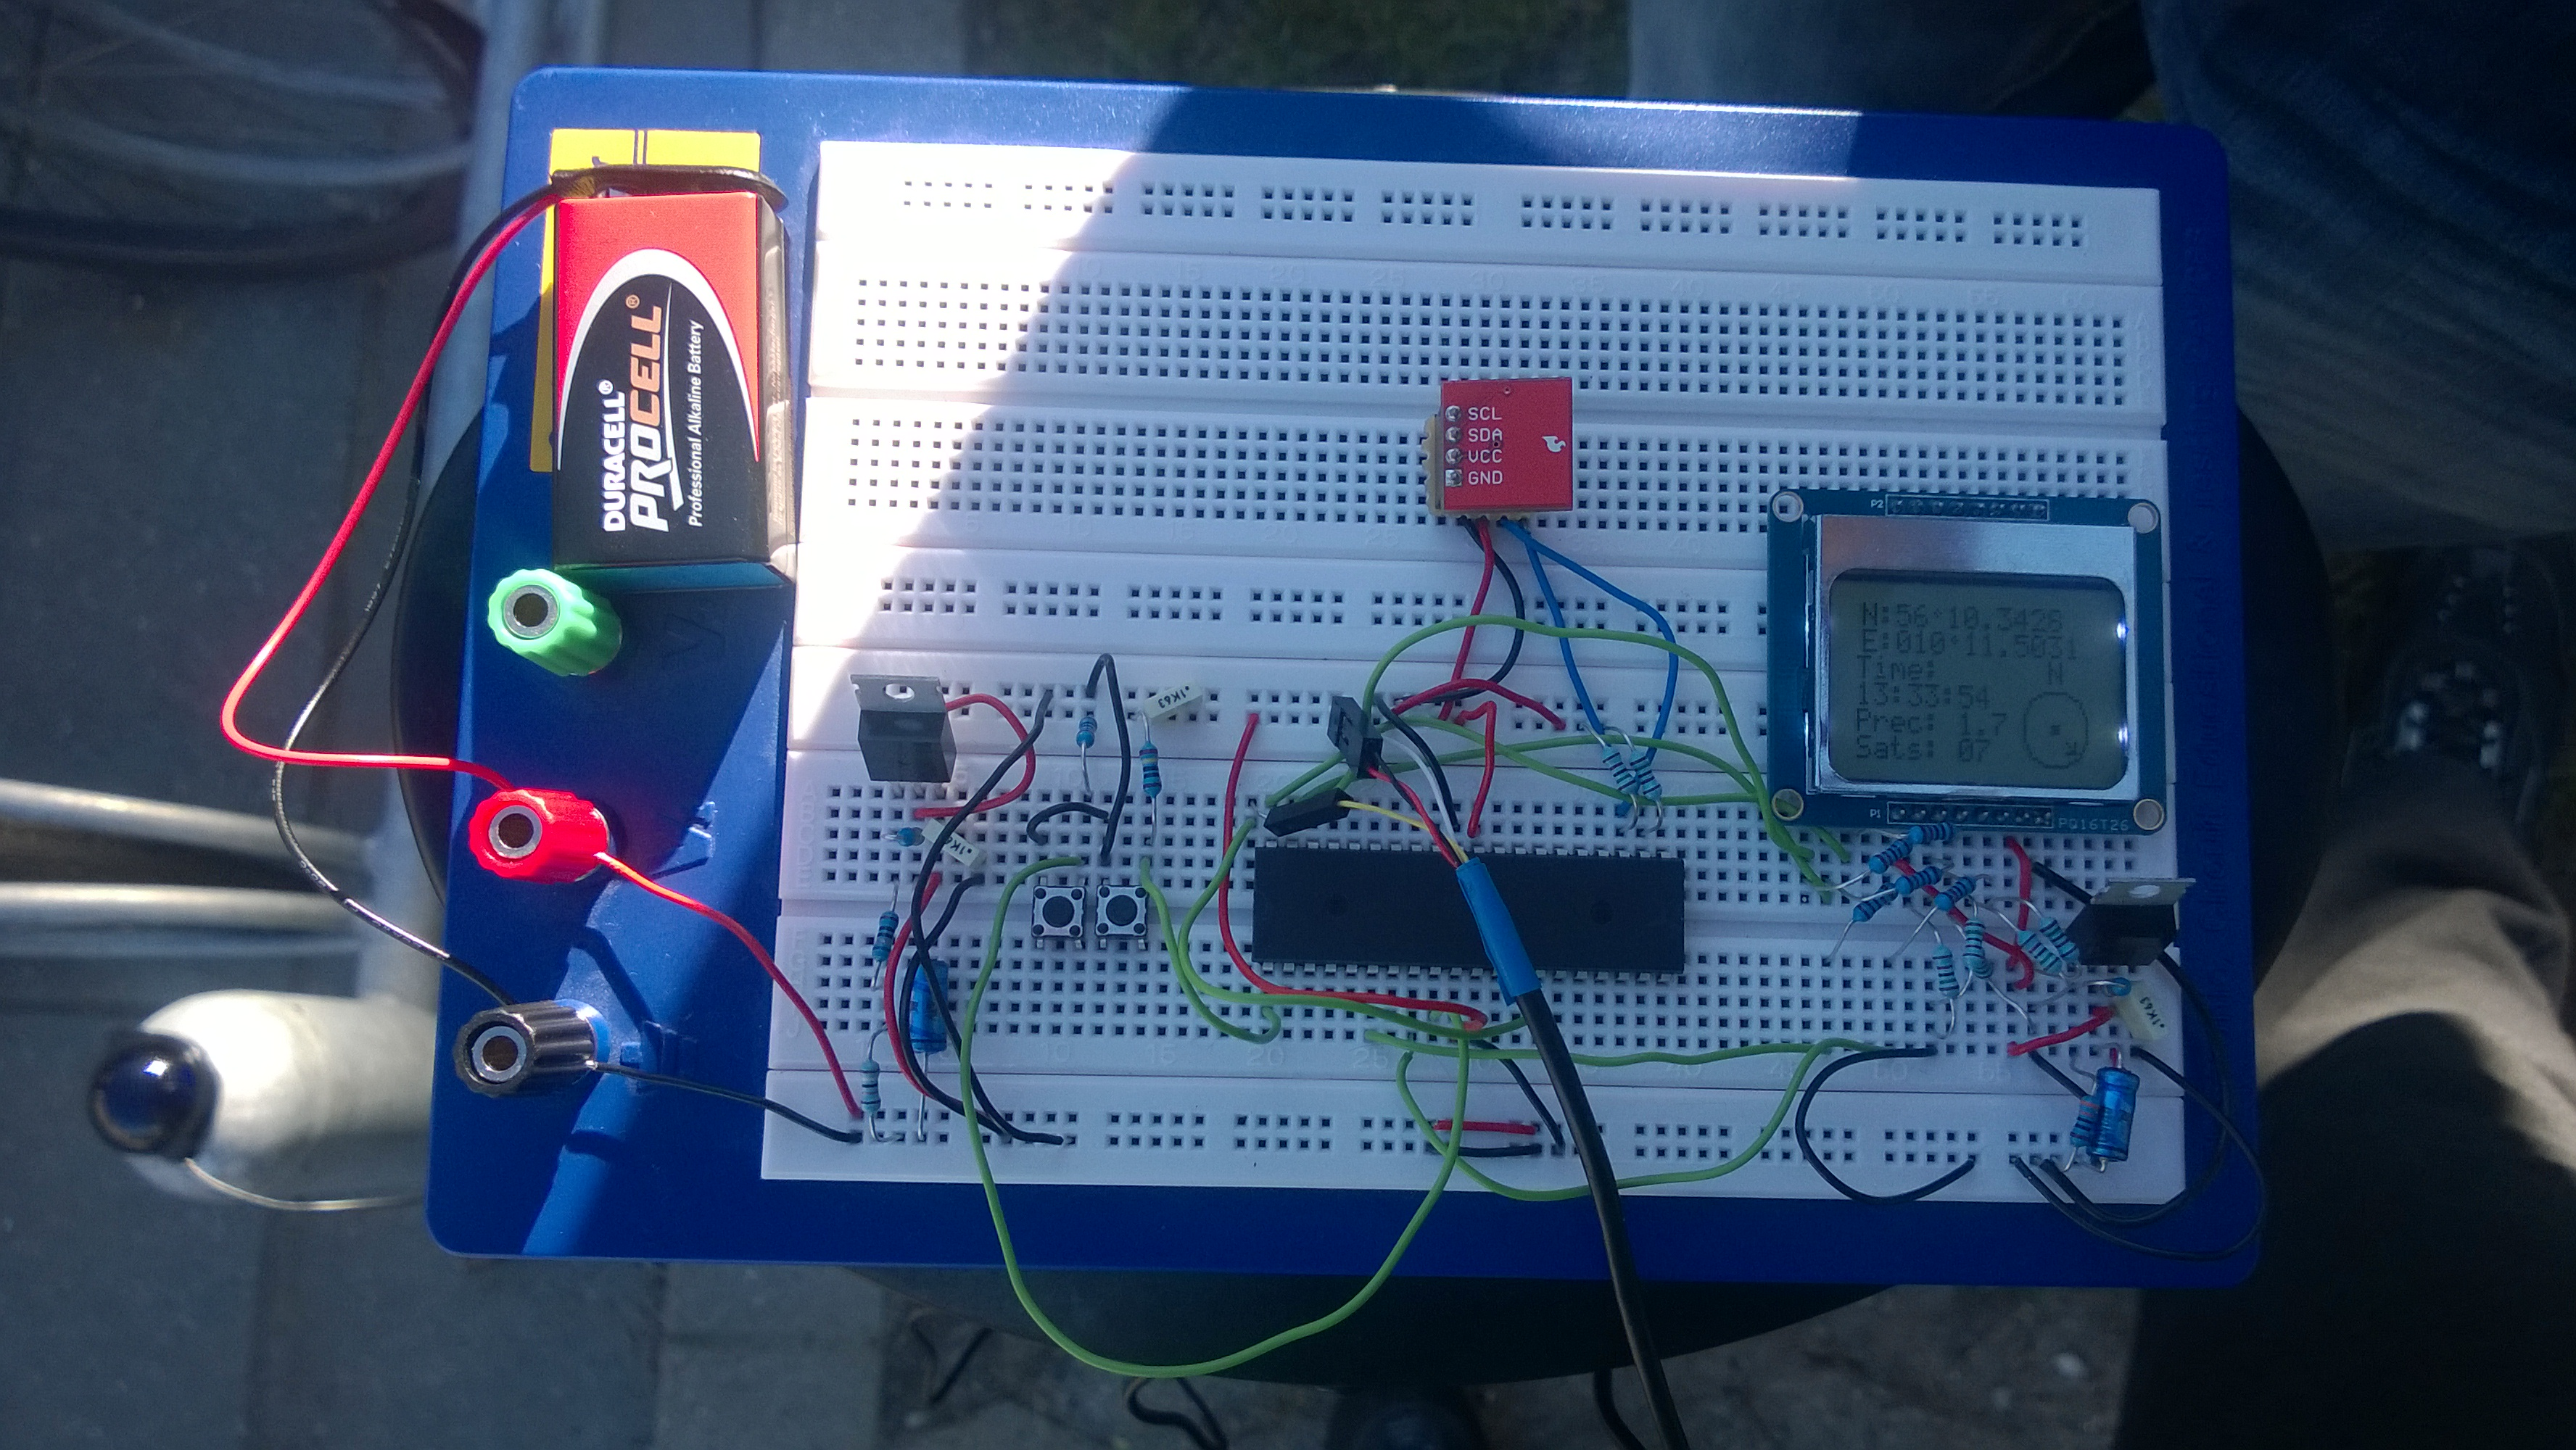
\includegraphics[width=.8\textwidth]{billeder/test_setup}
\caption{Picture of the test setup}
\end{figure}
On the picture the demobard is shown, and there is a clear read of the coordinates provided by the GPS module, which is seen as the black thing on the bicycle parking rack in the background.\\
The coordinates are:\\
$N:56^{\circ}10.3428$\\
$E:010^{\circ}11.5031$\\
Entering these coordinates in google maps we can get the location captured by the GPS module.

\begin{figure}[H]
\centering
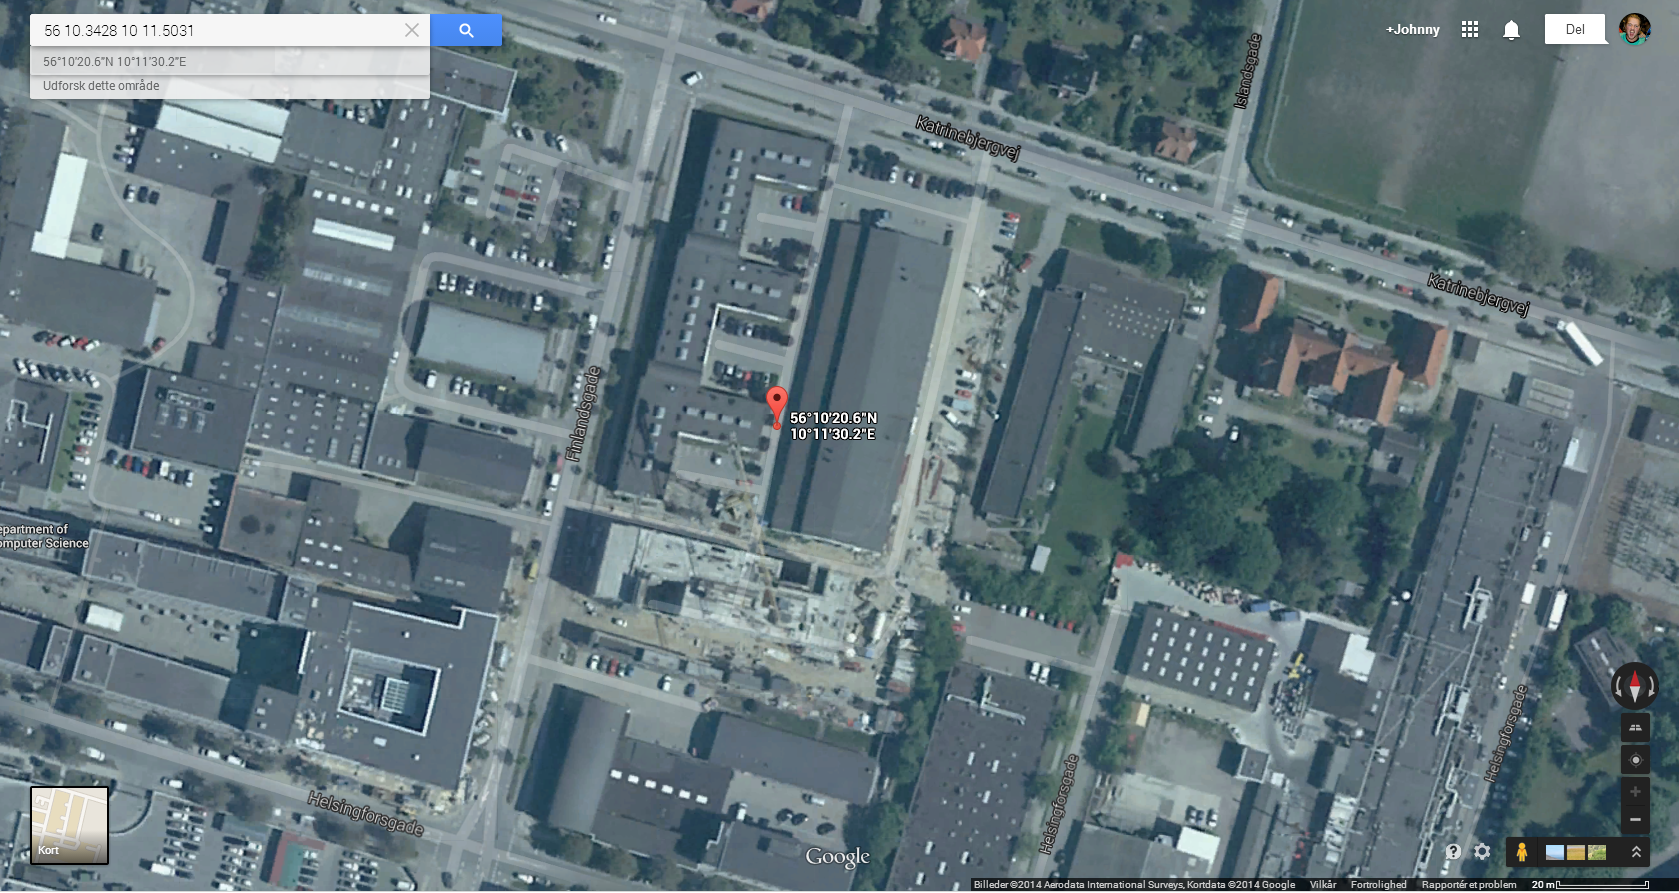
\includegraphics[width=.9\textwidth]{billeder/coordinate_map}
\caption{Test setup result plottet with google maps}
\end{figure}

In this test we had a precision of approx $\leq1$ meter.

\chapter{Improvements}
%Få RTOS optimeret
If we were to add hardware modules or features to our project we would have to look at the delay times in our RTOS tasks. Substantial work would go into optimising every task delay time to achieve the smoothest, most optimised system. This is something that can be done in the future. Adding RTOS elements like "suspend" and "resume" can further improve the system as there is no need to update the display if there is no new data as an example. \\

\chapter{Obtained experience}
\textbf{Screen:}\\
:)

\textbf{Magnetometer:}\\
hest

\textbf{GPS:}\\
By working with the GPS module we have acquired a working knowledge of the NMEA-0183 standard and how modules that utilise this standard work. 

\textbf{Boot Loader:}\\
When we first worked with bootloading it seemed simple enough, but after working with bootloading we have found out just how useful it is, as it saved us a lot of time and hassle.

\textbf{FreeRTOS:}\\
We have already worked with FreeRTOS in the exercise but implementing it in our own system has given us an understanding of the advantages of using a real time operating system. 





%%%%%%%%%%%%%%%%
%% konklusion %%
%%%%%%%%%%%%%%%%
\chapter{Conclusion}
We conclude on a successful project.


